% Copyright 2026 Sreeram Anil
% SPDX-License-Identifier: CC-BY-4.0
% =============================================================================
%  The electrochemical single-particle plant — foundational chapter
% =============================================================================
\chapter{The electrochemical single-particle plant}
\label{ch:spm}

The equivalent-circuit plant of \cref{ch:ecm} and the estimator model it faces share a structure:
both are an integrator plus two exponential lags plus a hysteresis state, and the differences
between them are parametric or additive. A benchmark built only on that pair measures how well a
filter handles noise, bias and parameter error --- but not how well it handles being \emph{wrong
about the physics}. This chapter describes the second plant, an electrochemical single-particle
model (SPM) that shares no state with the estimator's equivalent circuit, and quantifies the
structured model error it produces.

\section{Why a physics-based plant}
\label{sec:spm-why}

Battery models form a hierarchy of decreasing fidelity and increasing tractability
\cite{brosaplanella2022continuum}. At the top is the Doyle--Fuller--Newman (DFN) pseudo-two-dimensional
model \cite{doyle1993modeling}, which resolves lithium transport in the solid particles, in the
electrolyte and across the cell thickness; it is a coupled system of nonlinear
partial-differential equations and is what a cell designer uses. At the bottom is the
equivalent circuit: a handful of ordinary differential equations with empirical parameters,
which is what a BMS runs. The single-particle model sits between them. It retains solid-phase
diffusion --- the mechanism responsible for the slow relaxation that the $RC$ branches
\emph{imitate} --- and Butler--Volmer interfacial kinetics --- the mechanism responsible for the
nonlinear, rate-dependent overpotential that a linear resistor \emph{cannot} imitate --- while
discarding electrolyte transport and through-thickness variation. Formally it is the leading
order of an asymptotic expansion of the DFN model in the limit of fast electrolyte transport and
uniform reaction distribution, a derivation made rigorous by Marquis
et~al.~\cite{marquis2019spme}.

For this report the SPM occupies exactly the right rung. It is cheap enough to simulate at
\SI{0.1}{\second} for seventy estimators over nine scenarios and three seeds, it is a
\emph{different} model class from the estimator's circuit, and --- crucially --- it can be
cross-validated against an independent implementation, PyBaMM \cite{sulzer2021pybamm}, so that
the residual between plant and estimator is demonstrably the modelling gap rather than a bug.
The result is a benchmark in which every estimator faces a deterministic, structured,
load-correlated voltage error of a few millivolts that no amount of tuning can remove, which is
the regime in which real battery-management systems operate and in which the stochastic
assumptions of \cref{ch:prelim} are simply false.

\section{Governing equations}
\label{sec:spm-eqs}

Each electrode is represented by one spherical particle of radius $R_k$, $k\in\{\mathrm{n},\mathrm{p}\}$,
in which lithium moves by Fickian diffusion.

\subsection{Solid-phase diffusion}
Let $c_k(r,t)$ (\si{\mole\per\cubic\metre}) be the lithium concentration at radius $r$ in the
particle of electrode $k$. Then
\begin{equation}
\frac{\partial c_k}{\partial t}
 = \frac{1}{r^{2}}\frac{\partial}{\partial r}\!\left(r^{2}D_k\frac{\partial c_k}{\partial r}\right),
\qquad 0 < r < R_k,
\label{eq:spm-diffusion}
\end{equation}
with the symmetry condition at the centre and the flux condition at the surface,
\begin{equation}
\left.\frac{\partial c_k}{\partial r}\right|_{r=0} = 0,
\qquad
-D_k\left.\frac{\partial c_k}{\partial r}\right|_{r=R_k} = J_k .
\label{eq:spm-bc}
\end{equation}
$J_k$ (\si{\mole\per\square\metre\per\second}) is the molar flux leaving the particle surface.
It is obtained from the cell current by distributing the reaction uniformly over the interfacial
area of the electrode. With active-material volume fraction $\varepsilon_k$, coating thickness
$L_k$ and electrode area $A$, the specific interfacial area of a bed of spheres is
\begin{equation}
a_k = \frac{3\varepsilon_k}{R_k} \quad[\si{\per\metre}],
\label{eq:spm-area}
\end{equation}
and, with the discharge-positive convention of \cref{ch:ecm},
\begin{equation}
J_{\mathrm{n}} = \frac{+I}{F\,a_{\mathrm{n}}L_{\mathrm{n}}A},
\qquad
J_{\mathrm{p}} = \frac{-I}{F\,a_{\mathrm{p}}L_{\mathrm{p}}A} .
\label{eq:spm-flux}
\end{equation}
On discharge lithium leaves the graphite particle ($J_{\mathrm{n}}>0$) and enters the NMC
particle ($J_{\mathrm{p}}<0$), as it must.

\subsection{Interfacial kinetics}
The reaction at each particle surface is a one-electron charge transfer whose rate is related to
the surface overpotential by the Butler--Volmer equation \cite{newman2004}. With symmetric
transfer coefficients $\alpha_a = \alpha_c = 1/2$ the equation inverts in closed form,
\begin{equation}
\eta_k = \frac{2R_gT}{F}\,\operatorname{asinh}\!\left(\frac{F J_k}{2\,j_{0,k}}\right),
\label{eq:spm-bv}
\end{equation}
where $\eta_k$ (\si{\volt}) is the kinetic overpotential of electrode $k$ and $j_{0,k}$
(\si{\ampere\per\square\metre}) is the exchange-current density,
\begin{equation}
j_{0,k} = \kappa\,k_k(T)\,\sqrt{c_e}\,\sqrt{c_{k,\mathrm{surf}}}\,
 \sqrt{c_{\max,k}-c_{k,\mathrm{surf}}},
\qquad
k_k(T) = k_k\exp\!\left[\frac{E_{a,k}}{R_g}\left(\frac{1}{T_{\mathrm{ref}}}-\frac1T\right)\right].
\label{eq:spm-j0}
\end{equation}
Here $c_e$ is the (constant) electrolyte concentration, $c_{k,\mathrm{surf}}$ the solid
concentration at the particle surface, and $\kappa$ a design scaling introduced in
\cref{sec:spm-power} ($\kappa = 1$ reproduces the published parameters). Two structural
properties of \eqref{eq:spm-bv}--\eqref{eq:spm-j0} matter for estimation and have no counterpart
in an equivalent circuit:
\begin{itemize}[nosep,leftmargin=*]
\item $\operatorname{asinh}$ is linear only for $|FJ_k|\ll 2j_{0,k}$. Beyond that it is
  logarithmic, so the \emph{effective resistance} of the interface \emph{falls} as the current
  rises. This is the opposite of what a constant $R_0$ does and it is the single largest source of
  the residual in \cref{sec:spm-ident}.
\item $j_{0,k}$ vanishes at both ends of the stoichiometry range, $c_{\mathrm{surf}}\to 0$ and
  $c_{\mathrm{surf}}\to c_{\max}$, so the kinetic overpotential grows without bound as the
  electrode approaches full or empty. The equivalent circuit has no SOC-dependent resistance at
  all.
\end{itemize}
Note the sign of the Arrhenius exponent in \eqref{eq:spm-j0}: $j_0$ and the diffusivities are
\emph{transport} coefficients and therefore \emph{fall} when the cell is cooled, whereas the
resistances of \eqref{eq:ecm-arrhenius} \emph{rise}. The two conventions are reciprocal
expressions of the same activated physics.

\subsection{Terminal voltage and bulk SOC}
The terminal voltage is the difference of the two surface potentials, corrected by the kinetic
overpotentials and by a lumped ohmic resistance,
\begin{equation}
V = U_{\mathrm{p}}(y_{\mathrm{surf}}) + \eta_{\mathrm{p}}
  - U_{\mathrm{n}}(x_{\mathrm{surf}}) - \eta_{\mathrm{n}} - R_{\mathrm{ohm}}(T)\,I,
\label{eq:spm-voltage}
\end{equation}
where $x_{\mathrm{surf}} = c_{\mathrm{n,surf}}/c_{\max,\mathrm{n}}$ and
$y_{\mathrm{surf}} = c_{\mathrm{p,surf}}/c_{\max,\mathrm{p}}$ and $U_{\mathrm{n}},U_{\mathrm{p}}$
are the same electrode potentials \eqref{eq:ecm-Un}--\eqref{eq:ecm-Up} as in \cref{ch:ecm}. The
entropic coefficient \eqref{eq:ecm-entropic} is added to \eqref{eq:spm-voltage} split in equal
and opposite halves between the two electrodes, so that the full-cell temperature correction is
exactly \eqref{eq:ecm-ocvT}; the split itself has no physical content, it merely places the
correction where a per-electrode measurement would put it.

$R_{\mathrm{ohm}}$ collects everything the SPM does not model --- electrolyte ohmic drop, current
collectors, tabs and contact resistance --- as a single Arrhenius-scheduled series resistance,
\begin{equation}
R_{\mathrm{ohm}}(T) = R_{\mathrm{ohm}}^{\mathrm{ref}}
 \exp\!\left[\frac{E_{a,R}}{R_g}\left(\frac1T - \frac{1}{T_{\mathrm{ref}}}\right)\right],
\qquad E_{a,R} = \SI{20}{\kilo\joule\per\mole}.
\label{eq:spm-rohm}
\end{equation}

The state of charge is defined from the \emph{bulk} (volume-averaged) negative-electrode
stoichiometry through the same lithium balance \eqref{eq:ecm-xyz} used to build the OCV,
\begin{equation}
\bar{x} = \frac{1}{\tfrac43\pi R_{\mathrm{n}}^3}\int_0^{R_{\mathrm{n}}}
 \frac{c_{\mathrm{n}}(r)}{c_{\max,\mathrm{n}}}\,4\pi r^2\,\mathrm{d}r,
\qquad
\soc = 1 - \frac{x_{100}-\bar{x}}{\Delta x} .
\label{eq:spm-soc}
\end{equation}
This is the definition against which every estimator is scored on the SPM plant. It is the
\emph{bulk} SOC, not the surface one: a filter that tracks the surface stoichiometry perfectly
would still be wrong by several percent during a hover (\cref{sec:spm-surface}).

\subsection{Thermal coupling}
The plant carries the same lumped thermal state as the equivalent circuit,
\begin{equation}
C_{\mathrm{th}}\frac{\mathrm{d}T}{\mathrm{d}t}
 = I\big(U - V\big) - I\,T\,\frac{\partial U}{\partial T}(\soc)
 - \frac{T-T_{\mathrm{amb}}}{R_{\mathrm{th}}},
\label{eq:spm-thermal}
\end{equation}
with $U = \ocv(\soc,T)$ from \eqref{eq:ecm-ocv} and the sign convention derived in
\cref{sec:ecm-thermal}. The coupling runs both ways: $T$ scales $D_k$, $j_{0,k}$ and
$R_{\mathrm{ohm}}$, and those in turn set $V$ and hence the heat generation.

\section{Numerical scheme}
\label{sec:spm-numerics}

\eqref{eq:spm-diffusion} is discretised by finite volumes in $r$ and backward Euler in time, in
the form implemented in \code{plant\_spm.hpp} with $N_r = 20$ shells per particle.

\subsection{Control volumes}
Partition the particle into $N_r$ shells of equal thickness $\Delta r = R_k/N_r$, with shell $j$
occupying $[\,j\Delta r,\,(j{+}1)\Delta r\,]$ for $j = 0,\dots,N_r-1$. Dividing out the common
factor $4\pi$, the shell volume and the area of its outer face are
\begin{equation}
\mathcal{V}_j = \frac{r_{j+1}^3 - r_j^3}{3},
\qquad
\mathcal{A}_j = r_{j+1}^2,
\qquad r_j = j\Delta r .
\label{eq:spm-volumes}
\end{equation}
The unknown $c_j$ is the shell average, which to second order equals the value at the shell
centre $(j+\tfrac12)\Delta r$.

\subsection{Flux discretisation and time stepping}
Integrating \eqref{eq:spm-diffusion} over shell $j$ and applying the divergence theorem gives an
exact balance between the rate of change of the shell's content and the diffusive fluxes across
its two faces \cite{patankar1980}. Approximating each face flux by a two-point difference of the
neighbouring shell averages, and evaluating all fluxes at the new time level (backward Euler),
\begin{equation}
\mathcal{V}_j\,\frac{c_j^{n+1}-c_j^{n}}{\Delta t}
 = D\,\mathcal{A}_j\,\frac{c_{j+1}^{n+1}-c_j^{n+1}}{\Delta r}
 - D\,\mathcal{A}_{j-1}\,\frac{c_j^{n+1}-c_{j-1}^{n+1}}{\Delta r},
\label{eq:spm-fv}
\end{equation}
with the two boundary conditions \eqref{eq:spm-bc} imposed by setting the inner face flux of
shell $0$ to zero ($\mathcal{A}_{-1}\equiv0$) and replacing the outer face flux of shell
$N_r-1$ by the prescribed surface flux,
\begin{equation}
\mathcal{V}_{N_r-1}\,\frac{c_{N_r-1}^{n+1}-c_{N_r-1}^{n}}{\Delta t}
 = -\,D\,\mathcal{A}_{N_r-2}\,\frac{c_{N_r-1}^{n+1}-c_{N_r-2}^{n+1}}{\Delta r}
   \;-\; J\,R^2 .
\label{eq:spm-fv-surface}
\end{equation}
Collecting terms, \eqref{eq:spm-fv}--\eqref{eq:spm-fv-surface} is the tridiagonal system
\begin{equation}
-\ell_j\,c_{j-1}^{n+1} + \left(1+\ell_j+u_j\right)c_j^{n+1} - u_j\,c_{j+1}^{n+1} = c_j^{n} + s_j,
\qquad
\ell_j = \frac{\Delta t\,D\,\mathcal{A}_{j-1}}{\Delta r\,\mathcal{V}_j},
\quad
u_j = \frac{\Delta t\,D\,\mathcal{A}_{j}}{\Delta r\,\mathcal{V}_j},
\label{eq:spm-tridiag}
\end{equation}
with $\ell_0 = u_{N_r-1} = 0$ and the only non-zero source $s_{N_r-1} = -\Delta t\,J R^2/\mathcal{V}_{N_r-1}$.
It is solved in place by the Thomas algorithm \cite{thomas1949,golubvanloan2013} --- one forward
elimination and one back substitution, $\mathcal{O}(N_r)$ operations and no pivoting, which is
safe here because the matrix is strictly diagonally dominant by construction ($\ell_j,u_j>0$).
Backward Euler is unconditionally stable, which matters because the diffusive limit of an
explicit scheme, $\Delta t < \Delta r^2/(2D)$, is uncomfortably close to the sample period: for
the benchmark's power-cell geometry it is \SI{0.33}{\second} in the graphite particle at
\SI{25}{\celsius} and only \SI{0.15}{\second} at \SI{45}{\celsius}, against a
\SI{0.1}{\second} step --- a margin of \num{1.5}, and one that would shrink as $\Delta r^2$ with
any mesh refinement. The implicit step removes the constraint entirely and also allows the
identification tool of \cref{sec:spm-ident} to take much longer strides over rest periods.

\subsection{Surface concentration}
The finite-volume unknowns are shell averages; \eqref{eq:spm-voltage} needs the value \emph{at}
the surface. Reconstructing linearly within the outermost shell and using the flux boundary
condition \eqref{eq:spm-bc} to supply the gradient,
\begin{equation}
c_{\mathrm{surf}} = c_{N_r-1} + \frac{\Delta r}{2}
 \left.\frac{\partial c}{\partial r}\right|_{r=R}
 = c_{N_r-1} - \frac{J\,\Delta r}{2D} .
\label{eq:spm-csurf}
\end{equation}
The correction is exactly the concentration drop across half a shell under the quasi-steady
gradient, and it is first-order accurate in $\Delta r$. \cref{sec:spm-pybamm} shows that this
single approximation accounts for essentially the entire discrepancy against PyBaMM, and for all
of it at $t=0$.

\subsection{Conservation}
The scheme has an exact discrete conservation property, which is what makes the SOC definition
\eqref{eq:spm-soc} consistent with Coulomb counting to machine precision.

\begin{proposition}[Discrete lithium conservation]\label{prop:spm-conserve}
Summing \eqref{eq:spm-fv}--\eqref{eq:spm-fv-surface} over $j$, all interior face fluxes cancel in
pairs and
\begin{equation}
\sum_{j=0}^{N_r-1}\mathcal{V}_j\,\frac{c_j^{n+1}-c_j^{n}}{\Delta t} = -J R^2
\qquad\Longleftrightarrow\qquad
\frac{\mathrm{d}\bar{c}}{\mathrm{d}t} = -\frac{3J}{R},
\label{eq:spm-conserve}
\end{equation}
exactly, for any $N_r$ and any $\Delta t$, since $\sum_j\mathcal{V}_j = R^3/3$. Substituting
\eqref{eq:spm-area}--\eqref{eq:spm-flux} gives
$\mathrm{d}\bar{x}/\mathrm{d}t = -I/q_{\mathrm{n}}$ and hence, by \eqref{eq:ecm-dxdy} and
\eqref{eq:spm-soc},
\begin{equation}
\frac{\mathrm{d}\soc}{\mathrm{d}t} = -\frac{I}{3600\,Q_{\mathrm{nom}}} .
\label{eq:spm-coulomb}
\end{equation}
\end{proposition}

So the SPM plant's bulk SOC \emph{is} the Coulomb count, with no discretisation error and no
coulombic-efficiency loss. This is a deliberate property of the benchmark: on the SPM plant a
perfect Coulomb counter with a perfect current sensor would be exact, so everything an estimator
loses there is attributable to the voltage model, not to the SOC dynamics.

\section{Parameters}
\label{sec:spm-params}

\cref{tab:spm-params} lists the constants of the plant with their provenance. Most come from the
parameterisation of Chen et~al.~\cite{chen2020parameterization} for the LG~M50 cell as
distributed in the PyBaMM \texttt{Chen2020} set; the exceptions are flagged, and they matter
because the validation of \cref{sec:spm-pybamm} is only meaningful for the parameters that are
genuinely shared.

\begin{table}[H]\centering
\caption{Single-particle plant parameters. ``Chen 2020'' means the value is taken from
\cite{chen2020parameterization} as distributed in the PyBaMM \texttt{Chen2020} parameter set and
is therefore shared with the reference implementation used in \cref{sec:spm-pybamm};
``representative'' means the value is not in the published set and was chosen for this work.}
\label{tab:spm-params}
\begin{tabular}{llccl}\toprule
Quantity & Symbol & Negative & Positive & Source \\ \midrule
Particle radius & $R_k$ & \SI{5.86}{\micro\metre} & \SI{5.22}{\micro\metre} & Chen 2020\\
Active volume fraction & $\varepsilon_k$ & \num{0.75} & \num{0.665} & Chen 2020\\
Coating thickness & $L_k$ & \SI{85.2}{\micro\metre} & \SI{75.6}{\micro\metre} & Chen 2020\\
Electrode area & $A$ & \multicolumn{2}{c}{\SI{0.1027}{\square\metre}} & Chen 2020\\
Maximum concentration & $c_{\max,k}$ & \SI{33133}{\mole\per\cubic\metre} & \SI{63104}{\mole\per\cubic\metre} & Chen 2020\\
Solid diffusivity (\SI{25}{\celsius}) & $D_k$ & \SI{3.3e-14}{\square\metre\per\second} & \SI{4.0e-15}{\square\metre\per\second} & Chen 2020\\
Reaction-rate constant & $k_k$ & \num{6.48e-7} & \num{3.42e-6} & Chen 2020\\
Kinetic activation energy & $E_{a,k}$ & \SI{35}{\kilo\joule\per\mole} & \SI{17.8}{\kilo\joule\per\mole} & Chen 2020\\
Electrolyte concentration & $c_e$ & \multicolumn{2}{c}{\SI{1000}{\mole\per\cubic\metre}} & Chen 2020\\
Initial stoichiometry & $x_{100},y_{100}$ & \num{0.9014} & \num{0.2700} & Chen 2020\\
Nominal capacity & $Q_{\mathrm{nom}}$ & \multicolumn{2}{c}{\SI{5.0}{\ampere\hour}} & Chen 2020\\[1mm]
Diffusion activation energy & $E_{a,D_k}$ & \SI{30}{\kilo\joule\per\mole} & \SI{30}{\kilo\joule\per\mole} & representative\\
Lumped ohmic resistance & $R_{\mathrm{ohm}}^{\mathrm{ref}}$ & \multicolumn{2}{c}{\SI{5}{\milli\ohm} (benchmark)} & representative\\
Ohmic activation energy & $E_{a,R}$ & \multicolumn{2}{c}{\SI{20}{\kilo\joule\per\mole}} & representative\\
Lumped heat capacity & $C_{\mathrm{th}}$ & \multicolumn{2}{c}{\SI{70}{\joule\per\kelvin}} & \cite{lin2014thermal}\\
Thermal resistance & $R_{\mathrm{th}}$ & \multicolumn{2}{c}{\SI{3}{\kelvin\per\watt}} & \cite{lin2014thermal}\\
Radial shells & $N_r$ & \multicolumn{2}{c}{\num{20}} & ---\\
\bottomrule\end{tabular}
\end{table}

The two representative items are worth naming explicitly. The activation energies of the solid
diffusivities are \emph{not} part of the published Chen 2020 set, which was measured at
\SI{25}{\celsius}; \SI{30}{\kilo\joule\per\mole} is a conventional value for solid-state lithium
diffusion and is what gives the plant its temperature dependence. The lumped ohmic resistance is
likewise an addition: the SPM as such has no ohmic term, and PyBaMM's \texttt{Chen2020} set
contains a contact resistance of zero. The cross-validation of \cref{sec:spm-pybamm} therefore
sets $R_{\mathrm{ohm}}=0$, and the benchmark sets it to \SI{5}{\milli\ohm}.

\section{The power-cell design variant}
\label{sec:spm-power}

\subsection{What is scaled and why}
The LG~M50 is an \emph{energy} cell designed for a few C of peak discharge. An eVTOL aircraft
hovers at 4.5C \cite{yang2021evtol,fredericks2018vtol}. Running the published parameters at that
load does not produce a hard cell design; it produces a cell that is unusable, as
\cref{tab:spm-hover} shows. The benchmark therefore uses a \emph{power-cell design variant} of
the same chemistry, obtained by two geometric scalings and one lumped-parameter change:
\begin{equation}
R_k \leftarrow \rho\,R_k \ \ (\rho = 0.5),
\qquad
\kappa = 3,
\qquad
R_{\mathrm{ohm}}^{\mathrm{ref}} = \SI{5}{\milli\ohm}.
\label{eq:spm-scaling}
\end{equation}
Both scalings have a straightforward physical reading and neither changes the thermodynamics ---
the OCV, the capacity and the stoichiometry windows are untouched, so the two variants are the
same cell chemistry in a different electrode architecture.

\paragraph{Smaller particles.} Halving $R_k$ does two things at once. By \eqref{eq:spm-area} the
specific interfacial area $a_k = 3\varepsilon_k/R_k$ \emph{doubles}, from \SI{3.84e5}{\per\metre}
to \SI{7.68e5}{\per\metre} for the graphite, so the same cell current produces half the surface
flux $J_k$ and therefore a smaller kinetic overpotential. And the characteristic solid-diffusion
time $R_k^2/D_k$ falls by a factor of four, from \SI{1041}{\second} to \SI{260}{\second} for the
graphite and from \SI{6812}{\second} to \SI{1703}{\second} for the NMC, so concentration
gradients relax four times faster and the surface stoichiometry tracks the bulk much more
closely. This is precisely what electrode engineers do to build a power cell: thinner coatings,
finer particles, more surface area per ampere-hour, at a cost in volumetric energy density.

\paragraph{Faster kinetics.} $\kappa = 3$ multiplies the exchange-current density
\eqref{eq:spm-j0} threefold, representing a higher-rate active material and a better-conducting
interphase. Combined with the halved flux, the argument of the $\operatorname{asinh}$ in
\eqref{eq:spm-bv} falls by a factor of six at a given cell current.

\subsection{Kinetic overpotential: the published cell cannot hover}
\label{sec:spm-overpotential}
Evaluate \eqref{eq:spm-bv}--\eqref{eq:spm-j0} at $\soc = 0.9$ for both variants at 1C
($I=\SI{5}{\ampere}$) and at the 4.5C hover load ($I=\SI{22.5}{\ampere}$).
\cref{tab:spm-overpotential} collects the result. The published cell's exchange-current densities
at that operating point are $j_{0,\mathrm{n}} = \SI{0.263}{\ampere\per\square\metre}$ and
$j_{0,\mathrm{p}} = \SI{3.20}{\ampere\per\square\metre}$; the power variant's are
\SI{0.790}{} and \SI{9.61}{\ampere\per\square\metre}.

\begin{table}[H]\centering
\caption{Butler--Volmer overpotentials from \eqref{eq:spm-bv} at $\soc=0.9$, and the
\emph{effective} kinetic resistance $(\eta_{\mathrm{n}}-\eta_{\mathrm{p}})/I$ they imply. A
constant-parameter equivalent circuit must choose one value of this resistance for all currents.}
\label{tab:spm-overpotential}
\begin{tabular}{llcccc}\toprule
Variant & $T$ & rate & $\eta_{\mathrm{n}}$ [\si{\milli\volt}] & $\eta_{\mathrm{p}}$ [\si{\milli\volt}] & $R_{\mathrm{eff}}$ [\si{\milli\ohm}] \\ \midrule
published (\,$\rho{=}1,\kappa{=}1$)
 & \SI{25}{\celsius} & 1C   & $+90.5$  & $-13.4$ & \num{20.8} \\
 & \SI{25}{\celsius} & 4.5C & $+166.4$ & $-51.7$ & \num{9.7} \\
 & \SI{-10}{\celsius} & 1C   & $+163.8$ & $-29.0$ & \num{38.6} \\
 & \SI{-10}{\celsius} & 4.5C & $+231.9$ & $-83.6$ & \num{14.0} \\[1mm]
power variant (\,$\rho{=}0.5,\kappa{=}3$)
 & \SI{25}{\celsius} & 1C   & $+23.4$  & $-2.3$  & \num{5.1} \\
 & \SI{25}{\celsius} & 4.5C & $+76.9$  & $-10.1$ & \num{3.9} \\
 & \SI{-10}{\celsius} & 1C   & $+83.6$  & $-5.2$  & \num{17.8} \\
 & \SI{-10}{\celsius} & 4.5C & $+150.7$ & $-22.3$ & \num{7.7} \\
\bottomrule\end{tabular}
\end{table}

The last column is the crux of this chapter. For the published cell at \SI{25}{\celsius} the
effective kinetic resistance drops from \SI{20.8}{\milli\ohm} at 1C to \SI{9.7}{\milli\ohm} at
4.5C --- a factor of \num{2.1}. A constant resistor cannot span that: fitted to the low-rate data
it over-predicts the high-rate drop by more than \SI{250}{\milli\volt}, fitted to the high-rate
data it under-predicts the low-rate drop by \SI{55}{\milli\volt}. For the power variant the same
ratio is only \num{1.33} (\SIrange{5.1}{3.9}{\milli\ohm}), because the six-fold smaller
$\operatorname{asinh}$ argument keeps the kinetics in their near-linear regime over the whole
load range. \emph{The linear equivalent circuit is an adequate model of the power cell and an
inadequate model of the energy cell}, and \cref{sec:spm-ident} measures exactly how inadequate:
\SI{4.0}{\milli\volt} of residual root-mean-square error against \SI{24.1}{\milli\volt}.

\begin{table}[H]\centering
\caption{Terminal voltage of the two design variants under a sustained 4.5C hover from
$\soc_0=0.95$, isothermal, with their respective lumped ohmic resistances
(published: \SI{10}{\milli\ohm}; power: \SI{5}{\milli\ohm}). The cell reaches $\soc=0.856$ after
\SI{75}{\second}, the duration of the hover segment of the eVTOL mission; the open-circuit
voltage there is \SI{4.10}{\volt} and the cut-off is \SI{2.5}{\volt}.}
\label{tab:spm-hover}
\begin{tabular}{llccc}\toprule
Variant & $T$ & $V(0)$ [\si{\volt}] & $V(\SI{10}{\second})$ [\si{\volt}] & $V(\SI{75}{\second})$ [\si{\volt}] \\ \midrule
published & \SI{25}{\celsius}  & \num{3.643} & \num{3.605} & \num{3.430} \\
power     & \SI{25}{\celsius}  & \num{3.900} & \num{3.890} & \num{3.792} \\
published & \SI{-10}{\celsius} & \num{2.909} & \num{2.843} & \num{2.571} \\
power     & \SI{-10}{\celsius} & \num{3.580} & \num{3.528} & \num{3.336} \\
\bottomrule\end{tabular}
\end{table}

\cref{tab:spm-hover} settles the design question. At \SI{25}{\celsius} the published cell loses
\SI{690}{\milli\volt} --- \SI{17}{\percent} of its open-circuit voltage --- within a
\SI{75}{\second} hover starting from \SI{95}{\percent} SOC. At \SI{-10}{\celsius} it is at
\SI{2.57}{\volt} after \SI{75}{\second} and hits the \SI{2.5}{\volt} cut-off a few seconds later,
with \SI{86}{\percent} of its charge still in it. A pack built from such cells would have to be
oversized by a factor of three for the hover transient alone. The power variant ends the same
hover at \SI{3.79}{\volt} warm and \SI{3.34}{\volt} cold, which is a flyable design.

\section{Identification of the equivalent-circuit model}
\label{sec:spm-ident}

The estimators in the SPM benchmark are not given the electrochemical model; they are given the
same four-state equivalent circuit as in \cref{ch:ecm}, with parameters identified against the
SPM plant. This is exactly the industrial workflow --- characterise the cell, fit a circuit, ship
the circuit --- and it makes the plant/estimator gap a \emph{best-case} structured error rather
than an artificial one.

\subsection{Procedure}
The tool \code{tools/ident\_spm\_ecm.cpp} implements a dynamic-profile least-squares
identification, following \cite[Ch.~2]{plett2015bms1} and
\cite{hu2012comparative,ljung1999}.

\paragraph{Identification profile.} The SPM is simulated isothermally from
$\soc_0 = 0.95$ under a two-part excitation: first an HPPC-style pulse train of eight blocks,
each consisting of \SI{10}{\second} at 2C discharge, \SI{40}{\second} rest, \SI{10}{\second} at
1C charge, \SI{40}{\second} rest, a \SI{5}{\second} 4C pulse, \SI{40}{\second} rest, and finally
\SI{180}{\second} at 1C to step the SOC down by about \SI{5}{\percent}; then the full fixed-wing
mission profile with its gust process, which excites the model at realistic, correlated loads.
The record runs until $\soc<0.08$, about \SI{64}{\minute} at \SI{0.1}{\second} sampling.

\paragraph{Cost and parameterisation.} With $\vtheta = [R_0, R_1, \tau_1, R_2, \tau_2]^\T$,
\begin{equation}
J(\vtheta) = \sum_{k}\Big(v^{\mathrm{spm}}_k - v^{\mathrm{ecm}}_k(\vtheta)\Big)^2,
\label{eq:spm-cost}
\end{equation}
where the equivalent circuit is run \emph{open loop} over the same current record, with its SOC
obtained by Coulomb counting of that same current and its hysteresis magnitude set to
$M=0$ (the SPM has none). The OCV is shared by construction --- both models use
\eqref{eq:ecm-Un}--\eqref{eq:ecm-Up} --- so \eqref{eq:spm-cost} isolates the \emph{impedance}
mismatch and cannot be reduced by trading OCV against overpotential.

\paragraph{Optimisation.} \eqref{eq:spm-cost} is minimised by Levenberg--Marquardt
\cite{levenberg1944,marquardt1963}\cite[Ch.~10]{nocedal2006} over $\log\vtheta$, which enforces
positivity and equalises the scales of a resistance in milliohms and a time constant in hundreds
of seconds. Each iteration solves
\begin{equation}
\left(\bm{J}^\T\bm{J} + \lambda\,\diag(\bm{J}^\T\bm{J})\right)\bm{\delta}
 = \bm{J}^\T\bm{r},
\qquad \bm{r}_k = v^{\mathrm{spm}}_k - v^{\mathrm{ecm}}_k,
\label{eq:spm-lm}
\end{equation}
with the $n\times 5$ Jacobian $\bm{J}$ formed by central differences in log-space (step
$10^{-3}$), a full re-simulation per column. The damping $\lambda$ is divided by three on an
accepted step and multiplied by four on a rejected one, starting at $10^{-3}$; 40 iterations are
run.

\paragraph{Temperature dependence.} The whole fit is repeated isothermally at
$\SI{-10}{\celsius}$, \SI{10}{\celsius}, \SI{25}{\celsius} and \SI{45}{\celsius}, and each
parameter's activation energy is obtained by ordinary least squares of $\ln p$ on $1/T$, since
\eqref{eq:ecm-arrhenius} makes the slope exactly $E_a/R_g$.

\subsection{Identified parameters}
\cref{tab:spm-ident} gives the result for the power-cell variant used in the benchmark, which is
the parameter set \code{CellParams::ecm\_fitted\_to\_spm()} handed to every estimator, together
with the published-cell result for comparison.

\begin{table}[H]\centering
\caption{2-RC equivalent-circuit parameters identified against the SPM plant at
\SI{25}{\celsius}, with the activation energies from the four-temperature Arrhenius regression.
The benchmark uses the power-variant column.}
\label{tab:spm-ident}
\begin{tabular}{lcc}\toprule
 & power variant ($\rho{=}0.5$, $\kappa{=}3$, \SI{5}{\milli\ohm}) & published M50 ($\rho{=}\kappa{=}1$, \SI{10}{\milli\ohm}) \\ \midrule
$R_0$    & \SI{9.52}{\milli\ohm}  & \SI{23.83}{\milli\ohm} \\
$R_1$    & \SI{2.08}{\milli\ohm}  & \SI{4.69}{\milli\ohm} \\
$\tau_1$ & \SI{15.13}{\second} ($C_1 = \SI{7283}{\farad}$) & \SI{10.99}{\second} \\
$R_2$    & \SI{2.55}{\milli\ohm}  & \SI{18.46}{\milli\ohm} \\
$\tau_2$ & \SI{555.8}{\second} ($C_2 = \SI{218}{\kilo\farad}$) & \SI{562.7}{\second} \\[1mm]
residual RMSE, \SI{25}{\celsius} & \textbf{\SI{4.02}{\milli\volt}} & \textbf{\SI{24.09}{\milli\volt}} \\
residual RMSE, \SI{-10}{\celsius} & --- & \SI{139.8}{\milli\volt} \\
residual RMSE, \SI{45}{\celsius} & --- & \SI{10.6}{\milli\volt} \\[1mm]
$E_{a,R_0}$   & \SI{20.2}{\kilo\joule\per\mole} & \SI{16.5}{\kilo\joule\per\mole} \\
$E_{a,R_1}$   & \SI{17.1}{\kilo\joule\per\mole} & $-\SI{25.4}{\kilo\joule\per\mole}$ \\
$E_{a,R_2}$   & \SI{42.1}{\kilo\joule\per\mole} & \SI{34.5}{\kilo\joule\per\mole} \\
$E_{a,\tau}$  & $\approx 0$ (\SI{0.25}{} and $-\SI{2.5}{\kilo\joule\per\mole}$) & $-\SI{28.7}{}$, $-\SI{3.6}{\kilo\joule\per\mole}$ \\
\bottomrule\end{tabular}
\end{table}

Several features of \cref{tab:spm-ident} deserve comment.
\begin{itemize}[nosep,leftmargin=*]
\item $E_{a,R_0} = \SI{20.2}{\kilo\joule\per\mole}$ recovers, to within \SI{1}{\percent}, the
  \SI{20}{\kilo\joule\per\mole} that was put into $R_{\mathrm{ohm}}$ through
  \eqref{eq:spm-rohm}. The identification is consistent: the series resistance of the circuit is
  dominated by the lumped ohmic term of the plant, and the fit finds it.
\item $E_{a,R_2} = \SI{42.1}{\kilo\joule\per\mole}$ is \emph{larger} than any activation energy
  in the plant. The slow branch has to represent a diffusion impedance whose temperature
  dependence comes from $D_k$ \emph{and} whose magnitude grows because the surface depletion for
  a given flux scales as $J\sqrt{t/D}$; the circuit folds both into one resistance.
\item The time constants are essentially temperature-independent
  ($E_{a,\tau}\approx 0$, so the library sets $E_{a,\tau}=0$ exactly). Physically this is
  correct: the diffusion time is $R^2/D$ and is strongly temperature dependent, but the fit
  prefers to hold $\tau_2$ near \SI{556}{\second} --- a value lying between the two particles'
  diffusion times, \SI{260}{\second} and \SI{1703}{\second} --- and to put the entire
  temperature dependence into $R_2$. That is a legitimate re-parameterisation of the same
  impedance and a reminder that identified circuit parameters are not physical constants.
\item The published-cell fit produces a \emph{negative} $E_{a,R_1}$, i.e.\ a fast-branch
  resistance that grows with temperature. This is nonsense physically and is the signature of an
  over-stressed model: with a \SI{24}{\milli\volt} residual the optimiser is distributing
  unmodelled structure across whatever parameters will absorb it, and the parameters lose their
  meaning. It is the strongest argument for the power variant.
\end{itemize}

\subsection{The residual is structured, not white}
\label{sec:spm-residual}

\begin{figure}[H]\centering
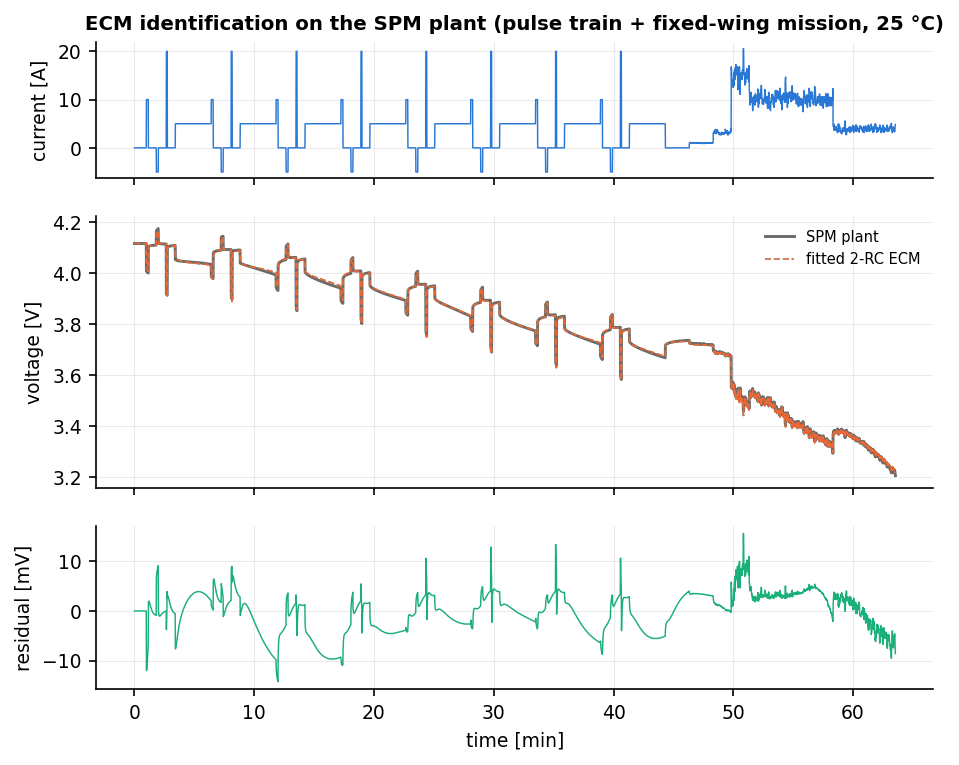
\includegraphics[width=\textwidth]{figures/model_spm_fit.png}
\caption{The identification record for the power-cell variant at \SI{25}{\celsius}. Top: the
current profile --- eight HPPC-style pulse blocks (2C discharge, 1C charge, 4C pulse, rests,
\SI{5}{\percent} SOC steps) followed by the fixed-wing mission with its gust process from
$t\approx\SI{50}{\minute}$. Middle: the SPM plant voltage and the fitted 2-RC equivalent circuit,
indistinguishable at this scale. Bottom: the residual, root-mean-square \SI{4.02}{\milli\volt},
with a peak of about \SI{15}{\milli\volt}. The residual is manifestly \emph{not} white: it
spikes at every current edge (the $\operatorname{asinh}$ kinetics), it drifts smoothly within
each rest (the diffusion tail that two exponentials cannot match), and it develops a systematic
negative trend below $\soc\approx0.2$ where $j_0$ collapses.}
\label{fig:spm-fit}
\end{figure}

\cref{fig:spm-fit} is the quantitative statement of the plant/estimator gap. Three distinct
structures are visible and each has an identifiable cause.
\begin{description}[nosep,leftmargin=*]
\item[Edge spikes.] At each current step the residual jumps by \SIrange{5}{15}{\milli\volt} and
  then decays. The equivalent circuit responds to a current step with an instantaneous
  $R_0\Delta i$ plus two exponentials; the SPM responds with an instantaneous
  $R_{\mathrm{ohm}}\Delta i$ plus a \emph{logarithmic} kinetic term plus a $\sqrt{t}$ diffusion
  term. The $\sqrt{t}$ short-time behaviour of semi-infinite diffusion has no exponential
  representation at all, and two time constants approximate it only over a limited band.
\item[Rate dependence.] Because $R_{\mathrm{eff}}$ falls with current (\cref{tab:spm-overpotential}),
  a single fitted $R_0$ is too small during the 4C pulses and too large during the 1C segments,
  with a sign flip in the residual between them.
\item[SOC dependence.] $j_{0,k}\propto\sqrt{c_{\mathrm{surf}}(c_{\max}-c_{\mathrm{surf}})}$ makes
  the kinetic overpotential grow near both ends of the range. The circuit has no
  SOC-dependent impedance, so the residual acquires a systematic drift at low SOC.
\end{description}

\begin{remark}[What \SI{4}{\milli\volt} of structured error is worth]\label{rem:spm-4mv}
By the error-gain relation \eqref{eq:ecm-errgain}, a voltage error $\delta v$ that the model
cannot represent is converted into an SOC error $\delta v/(\partial\ocv/\partial\soc)$. At the
mid-range slope of \SI{0.83}{\volt} a \SI{4}{\milli\volt} bias is worth \SI{0.5}{\percent} of
SOC; on the plateau at $\soc = 0.90$, where the slope is \SI{0.196}{\volt}, the same
\SI{4}{\milli\volt} is worth \SI{2.0}{\percent}. That single number explains the gap between the
two plants in Part~XIII: median steady-state SOC RMSE across all estimators is \num{0.0006} on
the nominal ECM scenario and \num{0.031} on the nominal SPM scenario, a factor of fifty.
\emph{And it is not noise.} Because the residual is deterministic and load-correlated, it
violates the whiteness assumption behind \eqref{eq:prelim-proc}--\eqref{eq:prelim-meas}: averaging
does not reduce it, a larger $\mR$ only slows the filter down without removing the bias, and
consistency tests (\cref{def:prelim-nis}) will report an inflated NIS no matter how the
covariances are tuned. The estimators that do best on this plant are the ones that either model
the error (augmented-state, disturbance and unknown-input observers), bound it (minimax and
set-membership methods) or discount it (fading-memory and robust weightings) --- not the ones
that estimate its variance.
\end{remark}

\section{Cross-validation against PyBaMM}
\label{sec:spm-pybamm}

An in-house plant is only as trustworthy as its verification. The estkit SPM was therefore
compared against PyBaMM \cite{sulzer2021pybamm}, the reference open-source battery-modelling
framework, using its \code{lithium\_ion.SPM} with the built-in \texttt{Chen2020} parameter set.
For the comparison both models are run with the \emph{published} parameters
($\rho=\kappa=1$), isothermally at \SI{25}{\celsius} and with zero contact resistance, so that
the two implementations share every physical parameter, every electrode potential function and
every initial stoichiometry. What remains is the numerical scheme: estkit uses $N_r = 20$
finite-volume shells with backward Euler at \SI{0.1}{\second}; PyBaMM uses its default
finite-volume mesh with an adaptive CasADi/IDAKLU differential-algebraic solver. The comparison
script is \code{scripts/validate\_pybamm.py}.

% Copyright 2026 Sreeram Anil
% SPDX-License-Identifier: CC-BY-4.0
\begin{table}[H]\centering\footnotesize\setlength{\tabcolsep}{4pt}\caption{Cross-validation of the estkit SPM plant (LG M50 parameters, isothermal \SI{25}{\celsius}, no contact resistance) against PyBaMM 26.8.0.0 \texttt{lithium\_ion.SPM} with the \texttt{Chen2020} parameter set: terminal-voltage differences over constant-current discharges from 100\,\% SOC.}\label{tab:val_pybamm}
\begin{tabular}{ccccc}\toprule C-rate & compared span [s] & RMSE [mV] & max $|\Delta v|$ [mV] & time to cut-off PyBaMM / estkit [s] \\ \midrule
0.5 & 7230 & 0.64 & 13.01 & 7230 / 7230 \\
1.0 & 3567 & 1.43 & 25.06 & 3567 / 3567 \\
2.0 & 1735 & 3.17 & 45.74 & 1735 / 1735 \\
\bottomrule\end{tabular}\end{table}


\begin{figure}[H]\centering
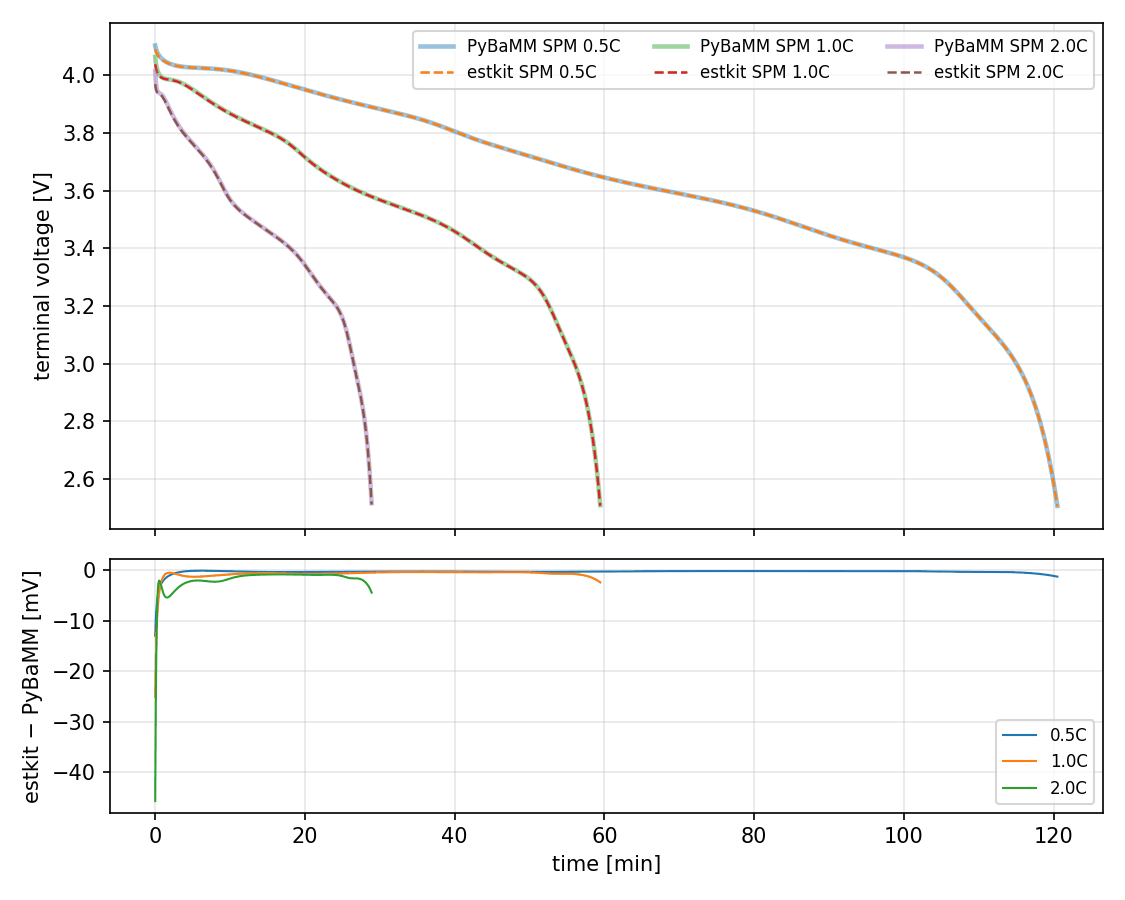
\includegraphics[width=\textwidth]{figures/validation_pybamm.png}
\caption{Constant-current discharges from \SI{100}{\percent} SOC to the \SI{2.5}{\volt} cut-off.
Top: the two implementations overlaid --- they are indistinguishable at plotting resolution over
the whole discharge, including the knee. Bottom: the difference. Apart from a transient in the
first seconds it stays within \SI{3}{\milli\volt} at every rate, and the discharge durations agree
exactly.}
\label{fig:spm-pybamm}
\end{figure}

\cref{tab:val_pybamm} and \cref{fig:spm-pybamm} give agreement of \SI{0.64}{}, \SI{1.43}{} and
\SI{3.17}{\milli\volt} root-mean-square at 0.5C, 1C and 2C, with \emph{identical} times to the
cut-off (\SI{7230}{}, \SI{3567}{} and \SI{1735}{\second}, to the \SI{1}{\second} output
resolution). Identical durations are the stronger of the two statements: they show that the two
codes agree on the total extractable charge and hence on the lithium balance, the stoichiometry
windows and the electrode potential functions --- everything thermodynamic. The millivolt-level
RMSE is then purely a statement about the kinetic and transport discretisation.

\paragraph{The initial transient.} The only sizeable discrepancy is a spike in the first few
seconds, reaching $-\SI{13.0}{}$, $-\SI{25.1}{}$ and $-\SI{45.7}{\milli\volt}$ at the three rates
and decaying within a minute. It is entirely explained by the surface reconstruction
\eqref{eq:spm-csurf}. At $t=0$ the particle is uniform, so the true surface concentration equals
the bulk value and the true concentration boundary layer has zero thickness; but
\eqref{eq:spm-csurf} imposes the \emph{quasi-steady} gradient $J/D$ across half a shell from the
very first sample. Evaluating that offset directly,
\begin{equation}
\Delta c_{\mathrm{surf}} = -\frac{J\,\Delta r}{2D},
\qquad
\Delta V = \big[U_{\mathrm{p}}(y_0+\delta y) - U_{\mathrm{p}}(y_0)\big]
 - \big[U_{\mathrm{n}}(x_0+\delta x) - U_{\mathrm{n}}(x_0)\big],
\label{eq:spm-initoffset}
\end{equation}
gives $\Delta V = -\SI{13.3}{}$, $-\SI{25.6}{}$ and $-\SI{47.2}{\milli\volt}$ at 0.5C, 1C and 2C
--- matching the observed maxima to within \SI{3}{\percent}, which identifies the mechanism
beyond doubt. The transient ends when the physical diffusion layer $\sqrt{Dt}$ grows past
$\Delta r/2$, which takes \SI{0.65}{\second} in the graphite ($\Delta r = \SI{0.293}{\micro\metre}$)
and \SI{4.3}{\second} in the NMC ($\Delta r = \SI{0.261}{\micro\metre}$, and $D_{\mathrm{p}}$
eight times smaller); thereafter the reconstruction is accurate and the two codes agree to better
than \SI{1}{\milli\volt}. The effect is a first-order artefact of $N_r=20$ and would shrink
proportionally with $\Delta r$; it is retained because $N_r=20$ is what makes the benchmark
affordable, and because a \SI{25}{\milli\volt} error confined to the first second of a
\SI{1}{\hour} discharge changes nothing an estimator sees.

\section{Surface versus bulk stoichiometry}
\label{sec:spm-surface}

The SPM's most consequential departure from an equivalent circuit is that it has two different
notions of ``state of charge''. The voltage is set by the \emph{surface} stoichiometry through
\eqref{eq:spm-voltage}; the SOC that the benchmark scores against is the \emph{bulk}
stoichiometry \eqref{eq:spm-soc}. Under load they differ, and the difference is a dynamic state
that the estimator's model represents only through its two $RC$ voltages.

\begin{figure}[H]\centering
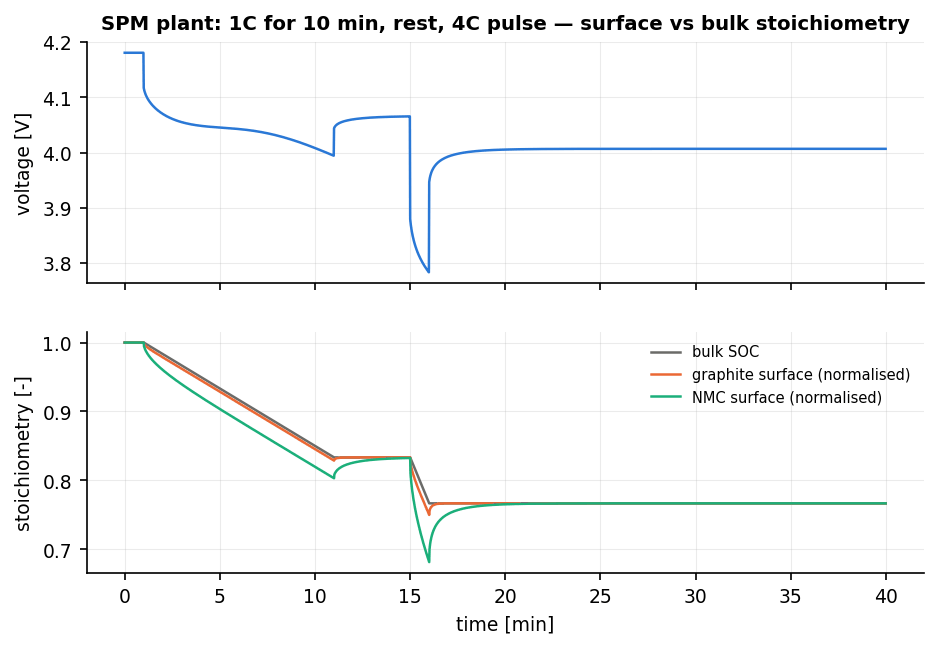
\includegraphics[width=\textwidth]{figures/model_spm_pulse.png}
\caption{Power-variant SPM under \SI{10}{\minute} at 1C, a \SI{4}{\minute} rest, a
\SI{1}{\minute} 4C pulse and a long rest. Top: terminal voltage. Bottom: bulk SOC
\eqref{eq:spm-soc} together with the two surface stoichiometries normalised onto the same scale.
The surface lags the bulk under load and relaxes towards it during rest; the NMC surface lags
much further than the graphite surface because its diffusivity is eight times smaller.}
\label{fig:spm-pulse}
\end{figure}

\cref{fig:spm-pulse} makes the gap quantitative. During the 1C segment the graphite surface runs
\num{0.005} of SOC-equivalent below the bulk while the NMC surface runs \num{0.030} below it. At
the end of the \SI{1}{\minute} 4C pulse the gaps are \num{0.017} and \num{0.085}: the cathode
surface is depleted by more than \emph{eight percentage points} of apparent SOC. On removal of
the load the graphite surface re-equilibrates in about \SI{40}{\second} while the NMC takes some
\SI{5}{\minute} to come within \num{0.002} of the bulk --- which is why the terminal voltage in
the top panel keeps climbing for minutes after the current is switched off, and why the
\SI{556}{\second} slow time constant of \cref{tab:spm-ident} came out where it did.

The estimation consequences are direct. First, an estimator that inverts the OCV at a
\SI{4}{\milli\volt} accuracy during or shortly after a high-rate segment is reading the surface,
not the bulk, and is biased low by up to \SI{8}{\percent} until the polarisation relaxes; the
$v_1,v_2$ states exist precisely to remove that bias, and they do it imperfectly because the
underlying process is a diffusion tail and not a sum of two exponentials. Second, the asymmetry
between the electrodes means the error has a \emph{long} component --- the slow branch, with a
time constant comparable to an entire cruise segment --- which is the state the observability
analysis of \cref{sec:ecm-obs} showed to be nearly collinear with the SOC itself
(\cref{tab:ecm-angle}: \ang{1.78} over a \SI{60}{\second} window at $\tau_2 = \SI{556}{\second}$).
A filter on the SPM plant must therefore separate two nearly indistinguishable directions using
a measurement that is biased by a structured \SI{4}{\milli\volt} error. That is the difficulty in
one sentence.

\section{What the SPM benchmark measures}
\label{sec:spm-mismatch}

The mismatches between the SPM plant and the estimators' equivalent circuit are structural rather
than parametric, and they are summarised in \cref{tab:spm-mismatch}.

\begin{table}[H]\centering
\caption{Structural differences between the single-particle plant and the four-state
equivalent-circuit model given to the estimators.}
\label{tab:spm-mismatch}
\begin{tabular}{p{38mm}p{45mm}p{50mm}}\toprule
Mechanism & SPM plant & Estimator model \\ \midrule
Interfacial kinetics & $\operatorname{asinh}$, rate- and SOC-dependent $j_0$ \eqref{eq:spm-bv} &
 constant $R_0$; effective resistance varies by \num{1.33} over the load range \\
Solid diffusion & PDE \eqref{eq:spm-diffusion}, $\sqrt{t}$ short-time response, $2\times20$ states &
 two exponentials, $\tau_1=\SI{15}{\second}$, $\tau_2=\SI{556}{\second}$ \\
Voltage-determining state & surface stoichiometry, lagging bulk by up to \num{0.085} &
 bulk SOC plus $v_1,v_2$ \\
Hysteresis & none & one-state model with $M = 0$ (correctly disabled) \\
Temperature & scales $D_k$, $j_{0,k}$, $R_{\mathrm{ohm}}$ separately &
 one Arrhenius factor per circuit element, $E_{a,\tau}=0$ \\
SOC dynamics & exact Coulomb count (\cref{prop:spm-conserve}) & exact Coulomb count \\
\bottomrule\end{tabular}
\end{table}

Because the SOC dynamics agree exactly, the SPM benchmark isolates one thing: \emph{the
estimator's ability to extract SOC from a voltage measurement that its own model mis-predicts by
a few structured millivolts.} The scenarios involving plant-side mechanisms that the SPM does not
have --- \code{preisach}, \code{aged\_cell}, and therefore \code{combined} --- are skipped, and
the remaining nine are run exactly as on the ECM plant.

The aggregate outcome, anticipating Part~XIII, is shown in \cref{tab:spm-scenariodiff}: on every
scenario the SPM plant is between twenty and fifty times harder than the ECM plant, and the
hardest of all is \code{cold}.

\begin{table}[H]\centering
\caption{Median steady-state SOC RMSE over all estimators, eVTOL mission, three seeds: the
equivalent-circuit plant against the single-particle plant.}
\label{tab:spm-scenariodiff}
\begin{tabular}{lcccccc}\toprule
Scenario & \code{nominal} & \code{init\_error} & \code{current\_bias} & \code{outliers} & \code{cold} & \code{hot} \\ \midrule
ECM plant & \num{0.0006} & \num{0.0008} & \num{0.0064} & \num{0.0018} & \num{0.0027} & \num{0.0003}\\
SPM plant & \num{0.0311} & \num{0.0352} & \num{0.0490} & \num{0.0183} & \num{0.0526} & \num{0.0199}\\
\bottomrule\end{tabular}
\end{table}

\paragraph{Why the cold case is hardest.} At \SI{-10}{\celsius} four effects compound, and only
the first exists on the ECM plant.
\begin{enumerate}[nosep,leftmargin=*]
\item \textbf{The overpotential grows and becomes more nonlinear.} By
  \cref{tab:spm-overpotential} the exchange-current densities fall by $6.5\times$ (graphite) and
  $2.6\times$ (NMC), so the $\operatorname{asinh}$ is driven further into its logarithmic regime:
  the effective kinetic resistance now spans \SIrange{17.8}{7.7}{\milli\ohm} between 1C and 4.5C,
  a ratio of \num{2.3} against \num{1.33} when warm. The constant-$R_0$ approximation degrades
  exactly where the model error is largest.
\item \textbf{The diffusion slows.} $D_k$ falls by a factor of \num{5.0} at
  \SI{30}{\kilo\joule\per\mole}, so the surface--bulk gap of \cref{sec:spm-surface} grows and
  relaxes more slowly, pushing yet more of the response into the slow branch --- the direction
  that \cref{tab:ecm-angle} identified as nearly unobservable over short windows.
\item \textbf{The circuit's temperature model is wrong in the wrong place.} The identified
  parameter set has $E_{a,\tau}=0$: the estimator's time constants do not change with
  temperature at all, while the plant's diffusion time constant grows by $6.5\times$. The whole
  temperature dependence has been loaded into $R_2$, which is a good approximation for the
  \emph{steady} response and a poor one for the \emph{transient} --- and a hover is all transient.
\item \textbf{The voltage window collapses.} The cell sits \SIrange{200}{400}{\milli\volt} lower
  under load, so the same absolute model error is a larger fraction of the usable range, and the
  plateau of \cref{fig:ecm-ocv} is traversed at a higher overpotential.
\end{enumerate}
This is also why the cold case is the right discriminator: it is not merely a harder version of
the nominal case but one in which the \emph{structure} of the model error changes, and filters
whose robustness depends on an assumption about the error's size --- rather than its shape ---
lose their advantage there. The extent to which cold-weather performance is a known and
persistent problem for lithium-ion traction batteries is documented at length by Jaguemont,
Boulon and Dub\'e \cite{jaguemont2016cold}.

\section{Summary}

The single-particle plant is a genuinely different model class from the estimator's equivalent
circuit: it resolves solid-phase diffusion in twenty shells per electrode, it computes the
interfacial overpotential from Butler--Volmer kinetics with a rate- and SOC-dependent
exchange-current density, and it sets the terminal voltage from the \emph{surface} stoichiometry
while the SOC to be estimated is the \emph{bulk} one. Its numerics conserve lithium exactly, so
its SOC is the Coulomb count to machine precision, and its voltage agrees with an independent
PyBaMM implementation of the same equations to \SIrange{0.6}{3.2}{\milli\volt} with identical
discharge durations. The power-cell design variant --- half the particle radius, three times the
kinetic rate constant, \SI{5}{\milli\ohm} of lumped ohmic resistance --- is what makes a 4.5C
hover possible at all and simultaneously what makes a constant-parameter equivalent circuit an
adequate model, reducing the best achievable 2-RC fit residual from \SI{24.1}{} to
\SI{4.0}{\milli\volt}. Those four millivolts are the point of the whole exercise: they are
deterministic, load-correlated and worth up to two percentage points of SOC on the OCV plateau,
and they are the error against which the seventy estimators of this report are measured when the
Gaussian assumptions of \cref{ch:prelim} no longer hold.
